\usepackage{hyperref}
\hypersetup{colorlinks=true,linkcolor=blue,pdfborderstyle={/S/U/W 1},
citecolor=red}
\usepackage[toc,page]{appendix}
\usepackage{mathtools}
\usepackage{amssymb}
\usepackage{axiom}
\usepackage{makeidx}
\usepackage{bussproofs} % for prooftree environment

\setlength{\textwidth}{400pt}
\makeindex
\usepackage{graphicx}
\usepackage{changepage} % for adjustwidth environment
\newwrite\sigfile

\begin{document}
\immediate\openout\sigfile=signatures.tex
\frontmatter
\setcounter{secnumdepth}{1}
\begin{titlepage}
\center{
\includegraphics{ps/axiomfront.ps}}
\vskip 0.1in
\includegraphics{ps/bluebayou.ps}\\
\vskip 0.1in
{\Huge{The 30 Year Horizon}}
\vskip 0.1in
$$
\begin{array}{lll}
Manuel\ Bronstein      & William\ Burge   & Timothy\ Daly \\
James\ Davenport       & Michael\ Dewar   & Martin\ Dunstan \\
Albrecht\ Fortenbacher & Patrizia\ Gianni & Johannes\ Grabmeier \\
Jocelyn\ Guidry        & Richard\ Jenks   & Larry\ Lambe \\
Michael\ Monagan       & Scott\ Morrison  & William\ Sit \\
Jonathan\ Steinbach    & Robert\ Sutor    & Barry\ Trager \\
Stephen\ Watt          & Jim\ Wen         & Clifton\ Williamson
\end{array}
$$
\center{\large{\VolumeName}}
\end{titlepage}
\pagenumbering{roman}
\begin{verbatim}
Portions Copyright (c) 2005 Timothy Daly

The Blue Bayou image Copyright (c) 2004 Jocelyn Guidry

Portions Copyright (c) 2004 Martin Dunstan
Portions Copyright (c) 2007 Alfredo Portes
Portions Copyright (c) 2007 Arthur Ralfs
Portions Copyright (c) 2005 Timothy Daly

Portions Copyright (c) 1991-2002, 
The Numerical ALgorithms Group Ltd.
All rights reserved.

This book and the Axiom software is licensed as follows:

Redistribution and use in source and binary forms, with or 
without modification, are permitted provided that the following 
conditions are
met:

    - Redistributions of source code must retain the above 
      copyright notice, this list of conditions and the 
      following disclaimer.

    - Redistributions in binary form must reproduce the above
      copyright notice, this list of conditions and the 
      following disclaimer in the documentation and/or other 
      materials provided with the distribution.

    - Neither the name of The Numerical ALgorithms Group Ltd. 
      nor the names of its contributors may be used to endorse 
      or promote products derived from this software without 
      specific prior written permission.

THIS SOFTWARE IS PROVIDED BY THE COPYRIGHT HOLDERS AND 
CONTRIBUTORS "AS IS" AND ANY EXPRESS OR IMPLIED WARRANTIES, 
INCLUDING, BUT NOT LIMITED TO, THE IMPLIED WARRANTIES OF 
MERCHANTABILITY AND FITNESS FOR A PARTICULAR PURPOSE ARE 
DISCLAIMED. IN NO EVENT SHALL THE COPYRIGHT OWNER OR 
CONTRIBUTORS BE LIABLE FOR ANY DIRECT, INDIRECT, INCIDENTAL, 
SPECIAL, EXEMPLARY, OR CONSEQUENTIAL DAMAGES (INCLUDING, 
BUT NOT LIMITED TO, PROCUREMENT OF SUBSTITUTE GOODS OR 
SERVICES; LOSS OF USE, DATA, OR PROFITS; OR BUSINESS 
INTERRUPTION) HOWEVER CAUSED AND ON ANY THEORY OF LIABILITY, 
WHETHER IN CONTRACT, STRICT LIABILITY, OR TORT (INCLUDING
NEGLIGENCE OR OTHERWISE) ARISING IN ANY WAY OUT OF THE USE 
OF THIS SOFTWARE, EVEN IF ADVISED OF THE POSSIBILITY OF 
SUCH DAMAGE.

\end{verbatim}

\vfill
\newpage
Inclusion of names in the list of credits is based on historical
information and is as accurate as possible. Inclusion of names
does not in any way imply an endorsement but represents historical
influence on Axiom development.

\begin{tabular}{lll}
Michael Albaugh        & Cyril Alberga          & Roy Adler\\
Christian Aistleitner  & Richard Anderson       & George Andrews\\
S.J. Atkins            & Jeremy Avigad          & Henry Baker\\
Martin Baker           & Stephen Balzac         & Yurij Baransky\\
David R. Barton        & Thomas Baruchel        & Gerald Baumgartner\\
Gilbert Baumslag       & Michael Becker         & Nelson H. F. Beebe\\
Jay Belanger           & David Bindel           & Fred Blair\\
Vladimir Bondarenko    & Mark Botch             & Raoul Bourquin\\
Alexandre Bouyer       & Karen Braman           & Wolfgang Brehm\\
Peter A. Broadbery     & Martin Brock           & Manuel Bronstein\\
Christopher Brown      & Stephen Buchwald       & Florian Bundschuh\\
Luanne Burns           & William Burge          & Ralph Byers\\
Quentin Carpent        & Pierre Casteran        & Robert Cavines\\
Bruce Char             & Ondrej Certik          & Tzu-Yi Chen\\
Bobby Cheng            & Cheekai Chin           & David V. Chudnovsky\\
Gregory V. Chudnovsky  & Mark Clements          & James Cloos\\
Jia Zhao Cong          & Josh Cohen             & Christophe Conil\\
Don Coppersmith        & George Corliss         & Robert Corless\\
Gary Cornell           & Meino Cramer           & Jeremy Du Croz\\
David Cyganski         & Nathaniel Daly         & Timothy Daly Sr.\\
Timothy Daly Jr.       & James H. Davenport     & David Day\\
James Demmel           & Didier Deshommes       & Michael Dewar\\
Inderjit Dhillon       & Jack Dongarra          & Jean Della Dora\\
Gabriel Dos Reis       & Claire DiCrescendo     & Sam Dooley\\
Zlatko Drmac           & Lionel Ducos           & Iain Duff\\
Lee Duhem              & Martin Dunstan         & Brian Dupee\\
Dominique Duval        & Robert Edwards         & Heow Eide-Goodman\\
Lars Erickson          & Mark Fahey             & Richard Fateman\\
Bertfried Fauser       & Stuart Feldman         & John Fletcher\\
Brian Ford             & Albrecht Fortenbacher  & George Frances\\
Constantine Frangos    & Timothy Freeman        & Korrinn Fu\\
Marc Gaetano           & Rudiger Gebauer        & Van de Geijn\\
Kathy Gerber           & Patricia Gianni        & Gustavo Goertkin\\
Samantha Goldrich      & Holger Gollan          & Teresa Gomez-Diaz\\
Laureano Gonzalez-Vega & Stephen Gortler        & Johannes Grabmeier\\
Matt Grayson           & Klaus Ebbe Grue        & James Griesmer\\
Vladimir Grinberg      & Oswald Gschnitzer      & Ming Gu\\
Jocelyn Guidry         & Gaetan Hache           & Steve Hague\\
Satoshi Hamaguchi      & Sven Hammarling        & Mike Hansen\\
Richard Hanson         & Richard Harke          & Bill Hart\\
Vilya Harvey           & Martin Hassner         & Arthur S. Hathaway\\
Dan Hatton             & Waldek Hebisch         & Karl Hegbloom\\
Ralf Hemmecke          & Henderson              & Antoine Hersen\\
Nicholas J. Higham     & Hoon Hong              & Roger House\\
Gernot Hueber          & Pietro Iglio           & Alejandro Jakubi\\
Richard Jenks          & Bo Kagstrom            & William Kahan\\
Kyriakos Kalorkoti     & Kai Kaminski           & Grant Keady\\
Wilfrid Kendall        & Tony Kennedy           & David Kincaid\\
Keshav Kini            & Ted Kosan              & Paul Kosinski\\
Igor Kozachenko        & Fred Krogh             & Klaus Kusche\\
\end{tabular}
\vfill
\newpage
\begin{tabular}{lll}
Bernhard Kutzler       & Tim Lahey              & Larry Lambe\\
Kaj Laurson            & Charles Lawson         & George L. Legendre\\
Franz Lehner           & Frederic Lehobey       & Michel Levaud\\
Howard Levy            & J. Lewis               & Ren-Cang Li\\
Rudiger Loos           & Craig Lucas            & Michael Lucks\\
Richard Luczak         & Camm Maguire           & Francois Maltey\\
Osni Marques           & Alasdair McAndrew      & Bob McElrath\\
Michael McGettrick     & Edi Meier              & Ian Meikle\\
David Mentre           & Victor S. Miller       & Gerard Milmeister\\
Mohammed Mobarak       & H. Michael Moeller     & Michael Monagan\\
Marc Moreno-Maza       & Scott Morrison         & Joel Moses\\
Mark Murray            & William Naylor         & Patrice Naudin\\
C. Andrew Neff         & John Nelder            & Godfrey Nolan\\
Arthur Norman          & Jinzhong Niu           & Michael O'Connor\\
Summat Oemrawsingh     & Kostas Oikonomou       & Humberto Ortiz-Zuazaga\\
Julian A. Padget       & Bill Page              & David Parnas\\
Susan Pelzel           & Michel Petitot         & Didier Pinchon\\
Ayal Pinkus            & Frederick H. Pitts     & Frank Pfenning\\
Jose Alfredo Portes    & E. Quintana-Orti       & Gregorio Quintana-Orti\\
Beresford Parlett      & A. Petitet             & Andre Platzer\\
Peter Poromaas         & Claude Quitte          & Arthur C. Ralfs\\
Norman Ramsey          & Anatoly Raportirenko   & Guilherme Reis\\
Huan Ren               & Albert D. Rich         & Michael Richardson\\
Jason Riedy            & Renaud Rioboo          & Jean Rivlin\\
Nicolas Robidoux       & Simon Robinson         & Raymond Rogers\\
Michael Rothstein      & Martin Rubey           & Jeff Rutter\\
Philip Santas          & Alfred Scheerhorn      & William Schelter\\
Gerhard Schneider      & Martin Schoenert       & Marshall Schor\\
Frithjof Schulze       & Fritz Schwarz          & Steven Segletes\\
V. Sima                & Nick Simicich          & William Sit\\
Elena Smirnova         & Jacob Nyffeler Smith   & Matthieu Sozeau\\
Ken Stanley            & Jonathan Steinbach     & Fabio Stumbo\\
Christine Sundaresan   & Klaus Sutner           & Robert Sutor\\
Moss E. Sweedler       & Eugene Surowitz        & Max Tegmark\\
T. Doug Telford        & James Thatcher         & Laurent Thery\\
Balbir Thomas          & Mike Thomas            & Dylan Thurston\\
Francoise Tisseur      & Steve Toleque          & Raymond Toy\\
Barry Trager           & Themos T. Tsikas       & Gregory Vanuxem\\
Kresimir Veselic       & Christof Voemel        & Bernhard Wall\\
Stephen Watt           & Andreas Weber          & Jaap Weel\\
Juergen Weiss          & M. Weller              & Mark Wegman\\
James Wen              & Thorsten Werther       & Michael Wester\\
R. Clint Whaley        & James T. Wheeler       & John M. Wiley\\
Berhard Will           & Clifton J. Williamson  & Stephen Wilson\\
Shmuel Winograd        & Robert Wisbauer        & Sandra Wityak\\
Waldemar Wiwianka      & Knut Wolf              & Yanyang Xiao\\
Liu Xiaojun            & Clifford Yapp          & David Yun\\
Qian Yun               & Vadim Zhytnikov        & Richard Zippel\\
Evelyn Zoernack        & Bruno Zuercher         & Dan Zwillinger\\
\end{tabular}
\newpage

\tableofcontents
\vfill
\eject
\setlength{\parindent}{0em}
\setlength{\parskip}{1ex}
{\Large{\bf New Foreword}}
\vskip .25in

On October 1, 2001 Axiom was withdrawn from the market and ended
life as a commercial product.
On September 3, 2002 Axiom was released under the Modified BSD
license, including this document.
On August 27, 2003 Axiom was released as free and open source
software available for download from the Free Software Foundation's
website, Savannah.

Work on Axiom has had the generous support of the Center for 
Algorithms and Interactive Scientific Computation (CAISS) at
City College of New York. Special thanks go to Dr. Gilbert 
Baumslag for his support of the long term goal.

The online version of this documentation is roughly 1000 pages.
In order to make printed versions we've broken it up into three
volumes. The first volume is tutorial in nature. The second volume
is for programmers. The third volume is reference material. We've
also added a fourth volume for developers. All of these changes
represent an experiment in print-on-demand delivery of documentation.
Time will tell whether the experiment succeeded.

Axiom has been in existence for over thirty years. It is estimated to
contain about three hundred man-years of research and has, as of
September 3, 2003, 143 people listed in the credits. All of these
people have contributed directly or indirectly to making Axiom
available.  Axiom is being passed to the next generation. I'm looking
forward to future milestones.

With that in mind I've introduced the theme of the ``30 year horizon''.
We must invent the tools that support the Computational Mathematician
working 30 years from now. How will research be done when every bit of
mathematical knowledge is online and instantly available? What happens
when we scale Axiom by a factor of 100, giving us 1.1 million domains?
How can we integrate theory with code? How will we integrate theorems
and proofs of the mathematics with space-time complexity proofs and
running code? What visualization tools are needed? How do we support
the conceptual structures and semantics of mathematics in effective
ways? How do we support results from the sciences? How do we teach
the next generation to be effective Computational Mathematicians?

The ``30 year horizon'' is much nearer than it appears.

\vskip .25in
%\noindent
Tim Daly\\
CAISS, City College of New York\\
November 10, 2003 ((iHy))
\vfill
\eject
\pagenumbering{arabic}
\setcounter{chapter}{1} % Chapter 1
